
\documentclass[runningheads]{llncs}
\usepackage[text={150mm,220mm},centering]{geometry}
\usepackage{graphicx}
\usepackage{tikz}
\usepackage{float}
\begin{document}
\title{\large{CSCI814 IT Project Management (Lab4)}}
%--------------------Please do NOT change the content above.-------------------------------------------------

%
%----Please write your personal information as below.------------------------------------
%
\author{\large{Student Name: Wangzhihui Mei \\ % Please write your name here
CCNU Student Number: 2019124044 \\ % Please write your CCNU student number here
UOW Student Number: 6603385}}  % Please write your UOW student number here


%-----------------------------------------------------------------------------------------------



%---------Do not change the content of this part--------------------

\authorrunning{CCNU Wollongong Joint Institute}
\institute{Central China Normal University Wollongong Joint Institute}

\maketitle
\clearpage

%-----------Please write your solutions to the questions in the assignment from here.---------------

\section*{In-class}
\subsection*{3. SimpleTrackBaseline}
\begin{figure}[H]
    \centering
    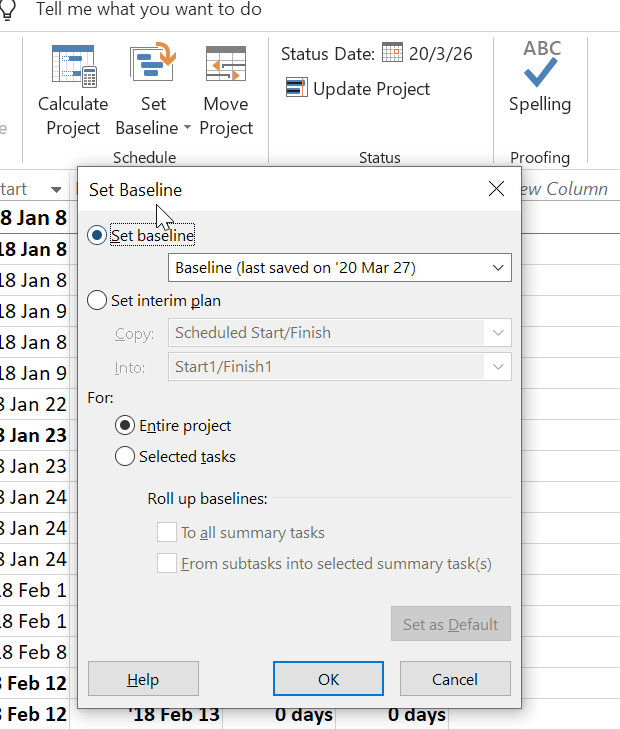
\includegraphics[width=0.5\textwidth]{./image/t2f1}
    \caption{Set Baseline}
\end{figure}

\begin{figure}[H]
    \centering
    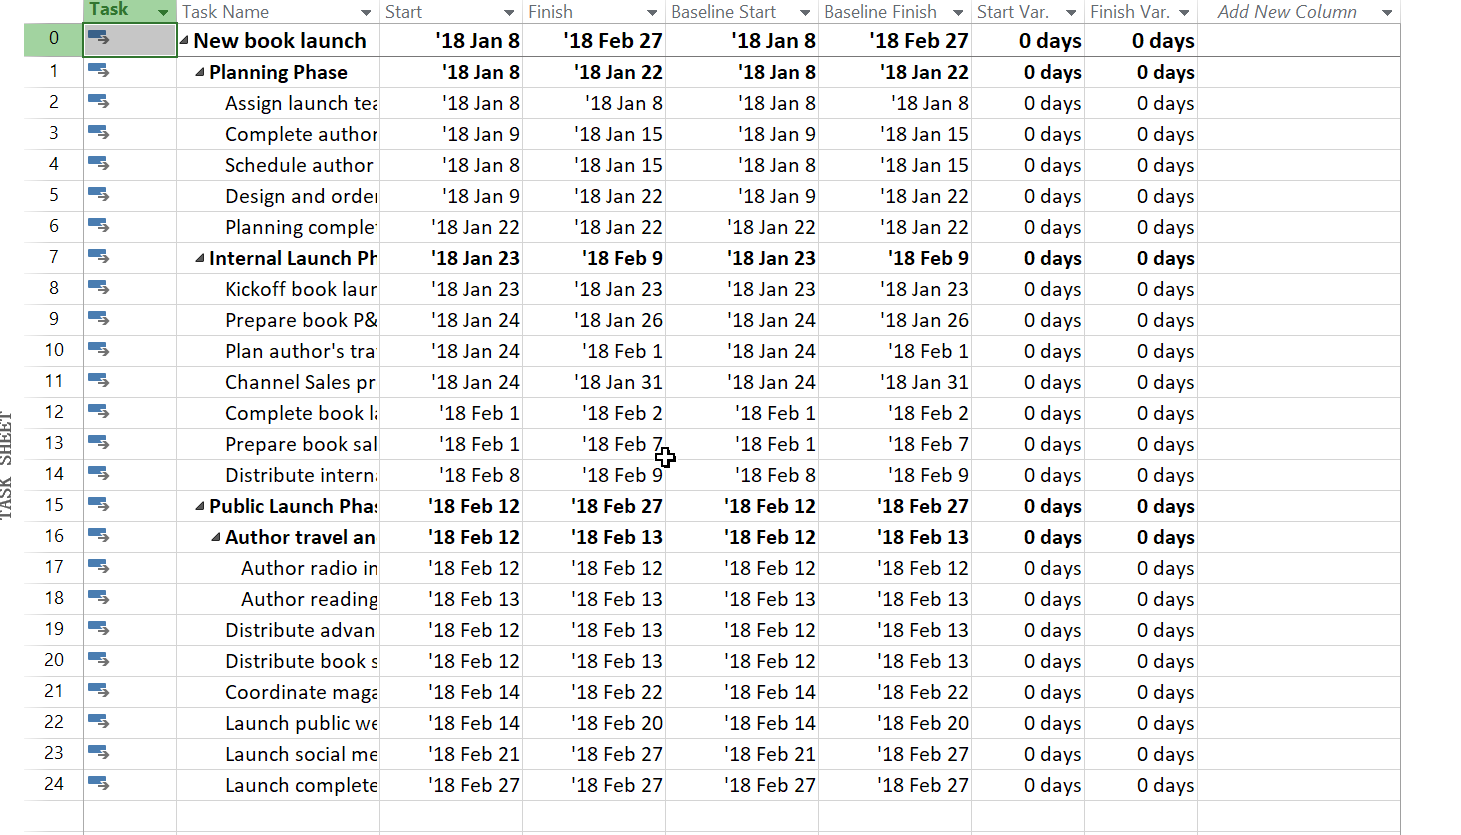
\includegraphics[width=0.9\textwidth]{./image/t2f2}
    \caption{Variance between scheduled and baseline values}
\end{figure}

No variance between the scheduled and baseline values.

\subsection*{4. SimpleTrackActuals}
\begin{figure}[H]
    \centering
    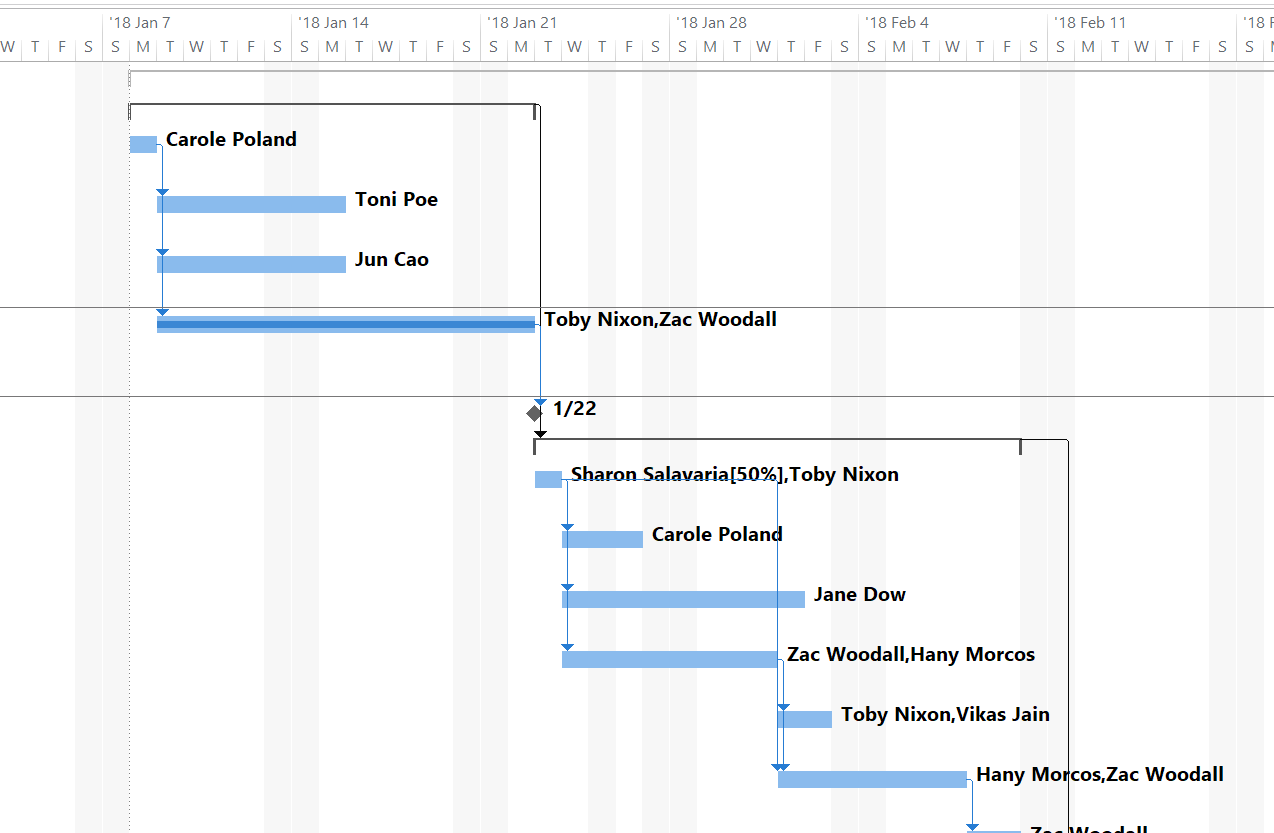
\includegraphics[width=0.9\textwidth]{./image/t3f1}
    \caption{Gantt Chart}
\end{figure}

The "Design and order marketing material" task is the deterministic task.

\begin{figure}[H]
    \centering
    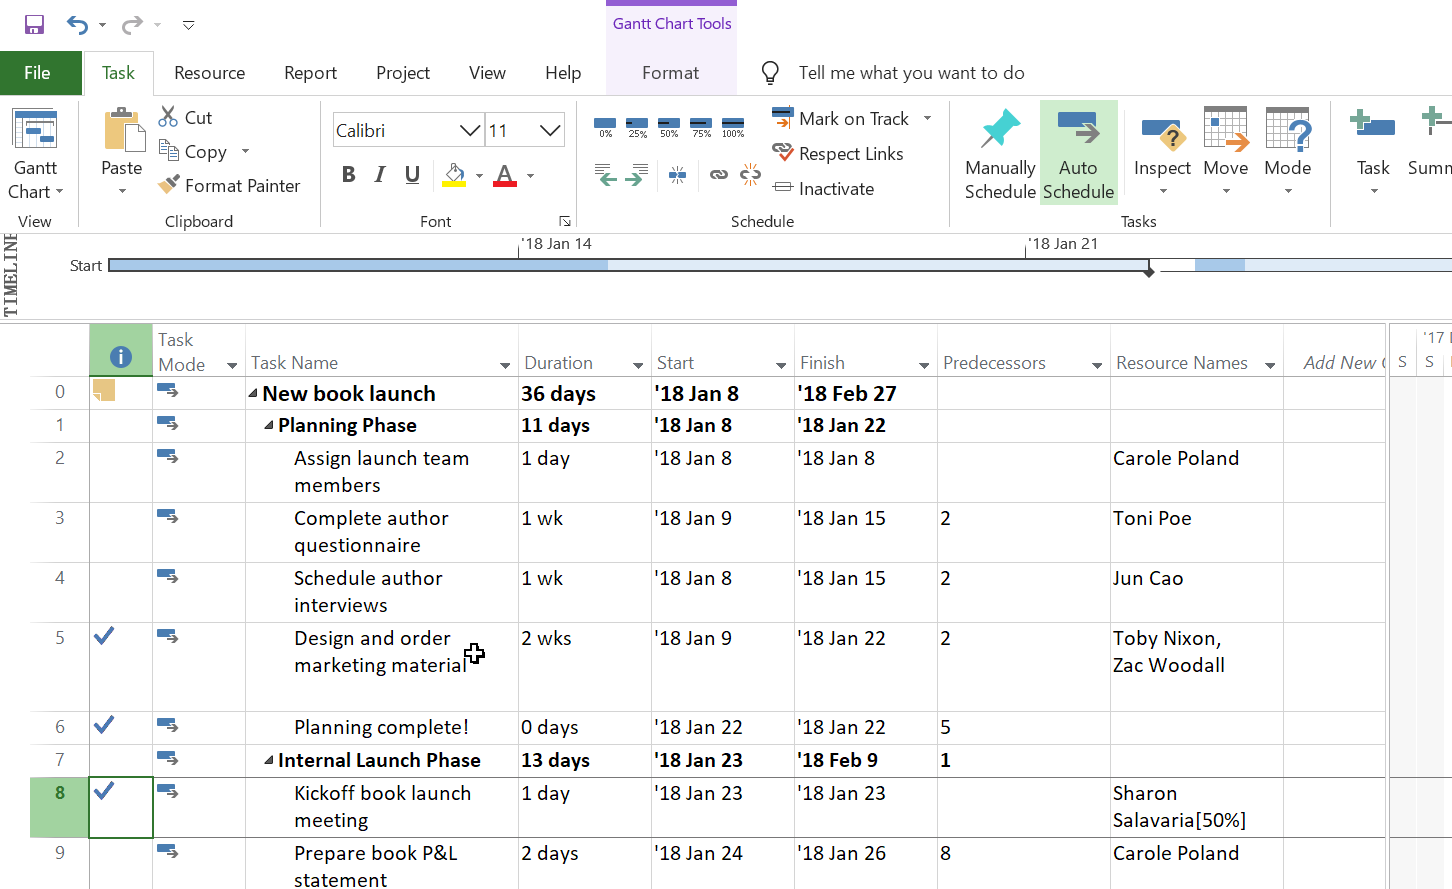
\includegraphics[width=0.9\textwidth]{./image/t3f2}
    \caption{b}
\end{figure}

\begin{figure}[H]
    \centering
    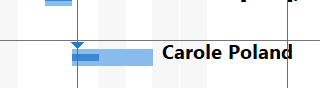
\includegraphics[width=0.9\textwidth]{./image/t3f3}
    \caption{c}
\end{figure}

\begin{figure}[H]
    \centering
    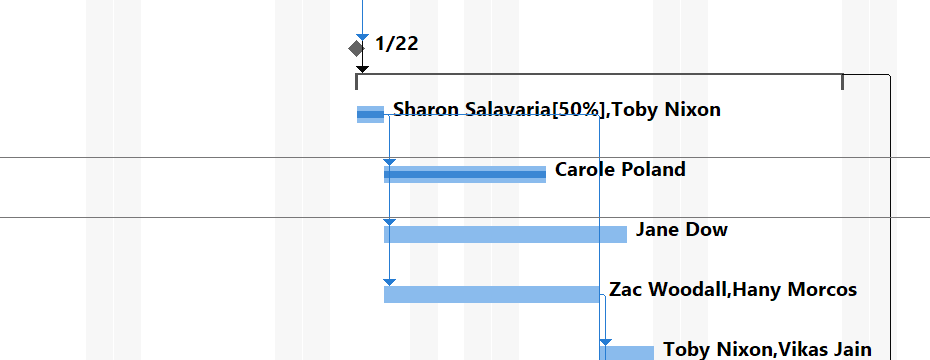
\includegraphics[width=0.9\textwidth]{./image/t3f4}
    \caption{di. The bar become longer}
\end{figure}

\begin{figure}[H]
    \centering
    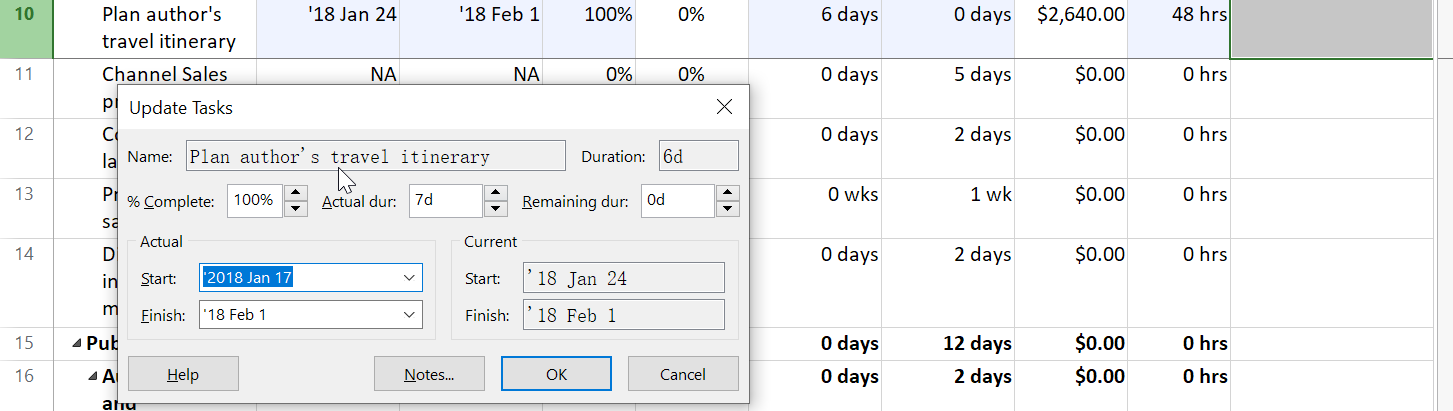
\includegraphics[width=0.9\textwidth]{./image/t3f5}
    \caption{dii. Update the task 10}
\end{figure}


\begin{figure}[H]
    \centering
    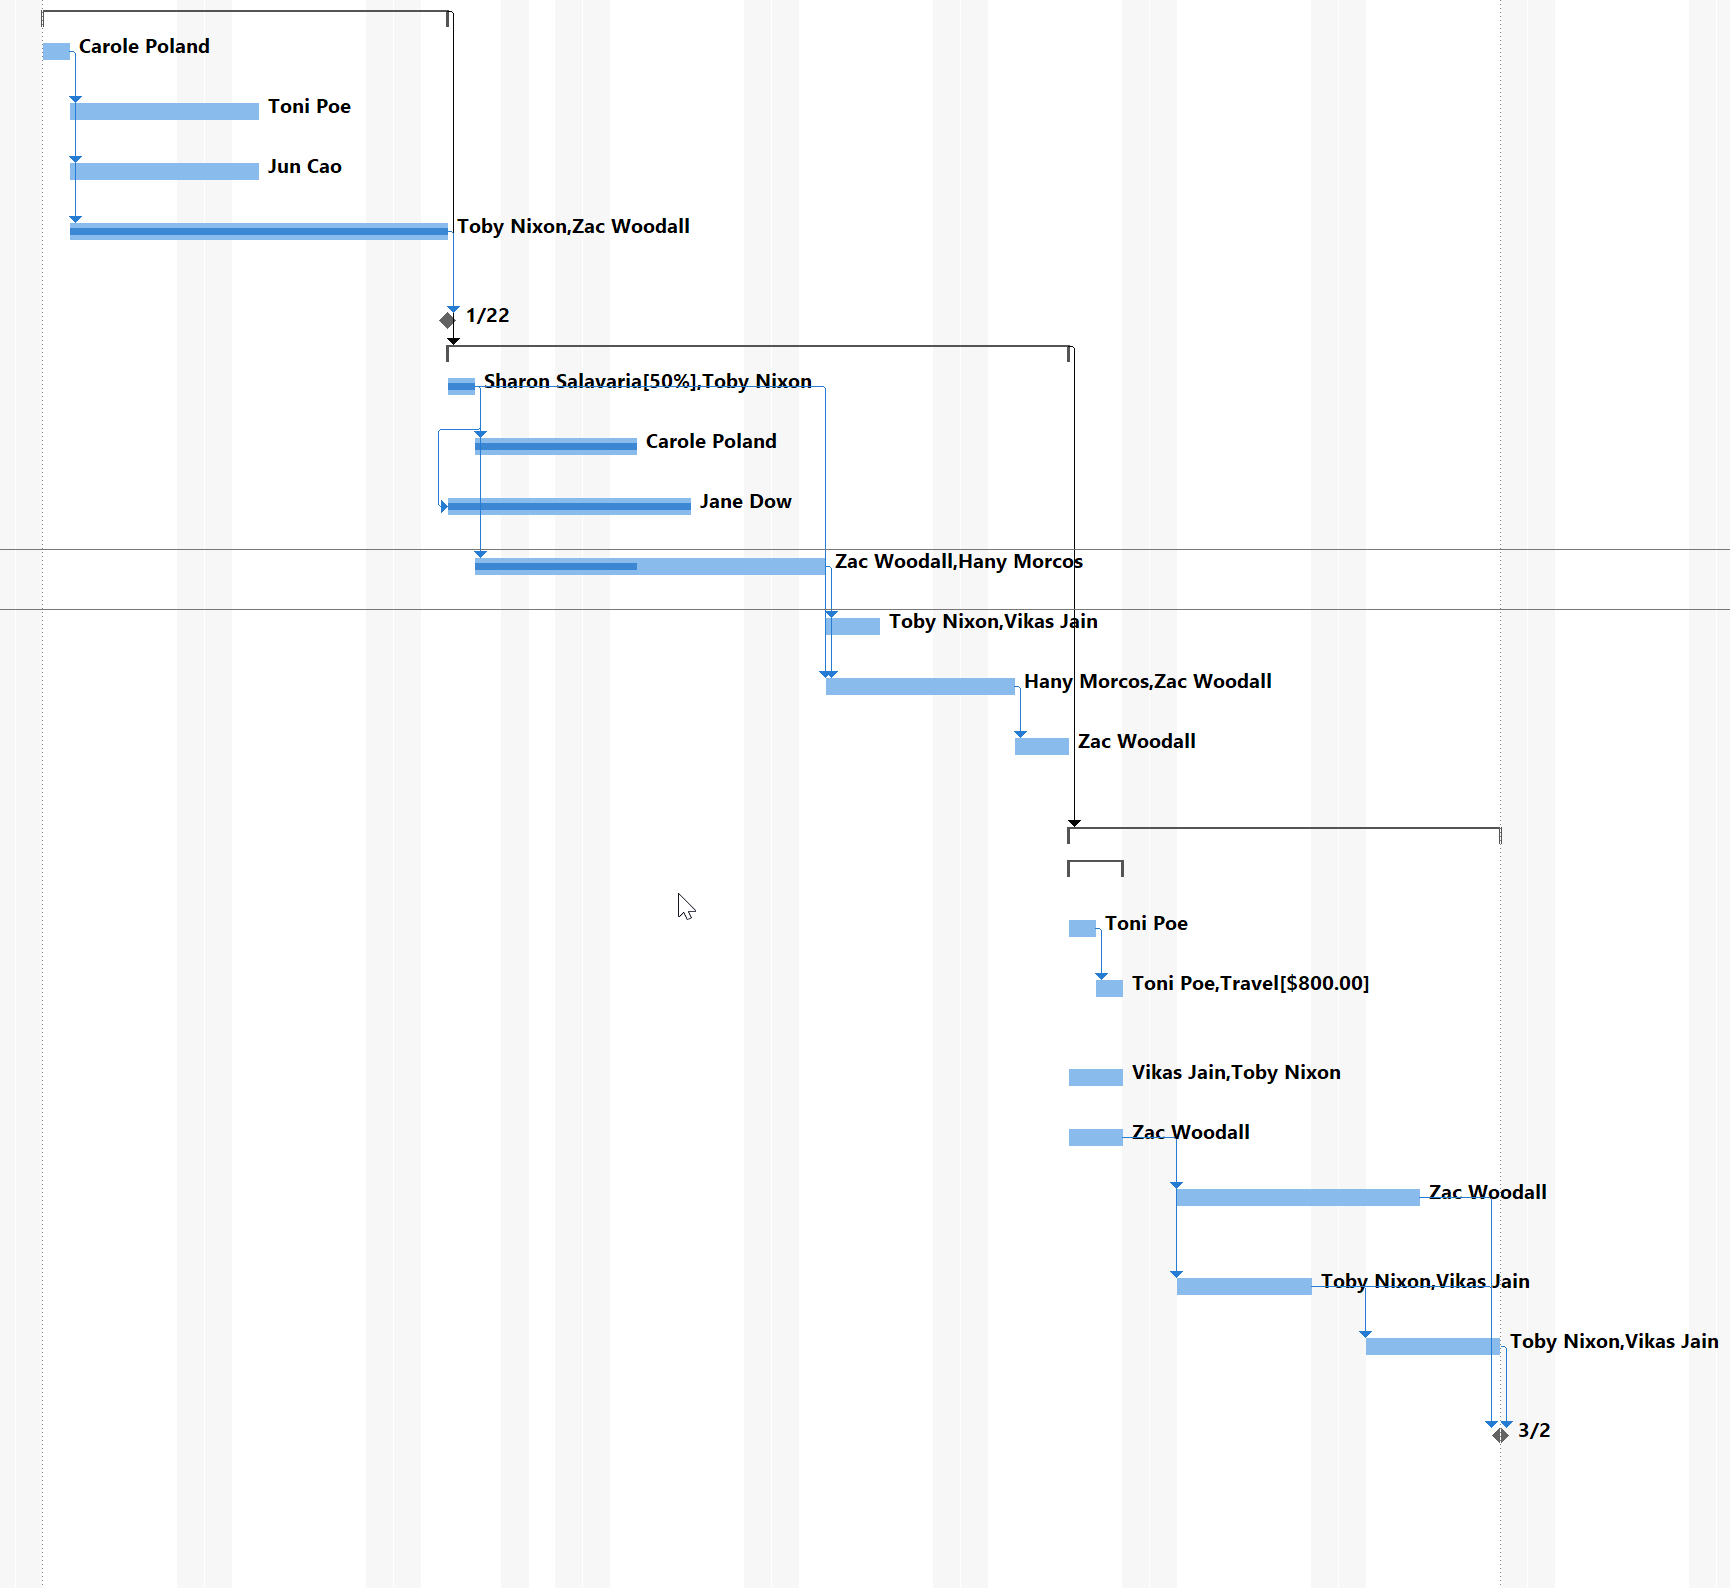
\includegraphics[width=0.9\textwidth]{./image/t3f6}
    \caption{diii. Update the task 11}
\end{figure}

New finish date of the project is March 2.

\clearpage
\section*{Lab4}
\subsection*{5. Updatebaseline}
\begin{figure}[H]
    \centering
    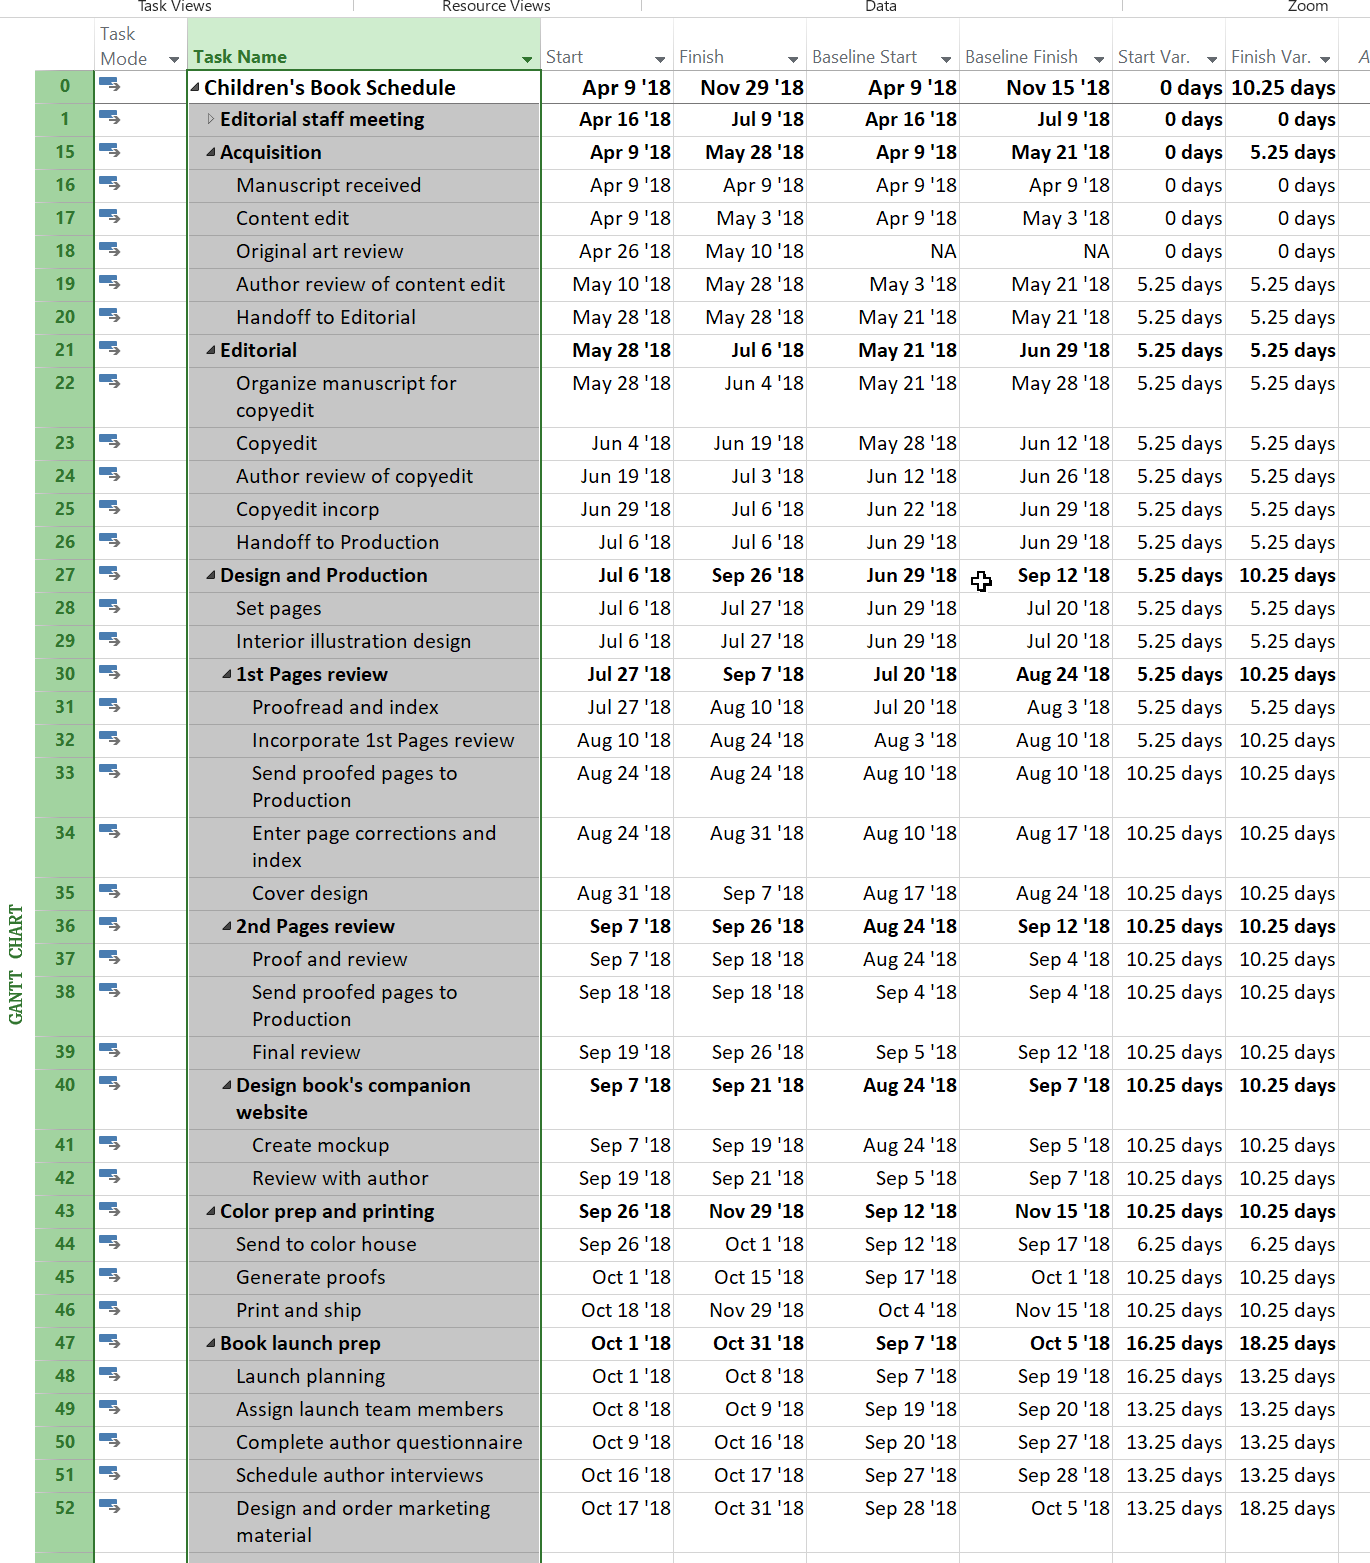
\includegraphics[width=0.9\textwidth]{./image/t4f1}
    \caption{Variance between baseline and task}
\end{figure}

There are several tasks actuals vary with the schedule.

\subsection*{6. TrackWork}
\begin{figure}[H]
    \centering
    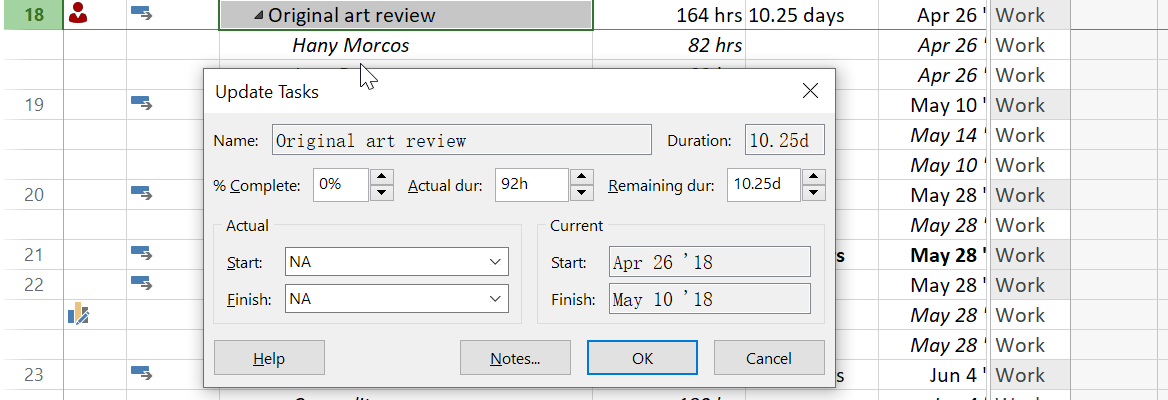
\includegraphics[width=0.9\textwidth]{./image/t5f1}
    \caption{Change Actual Work}
\end{figure}
\begin{figure}[H]
    \centering
    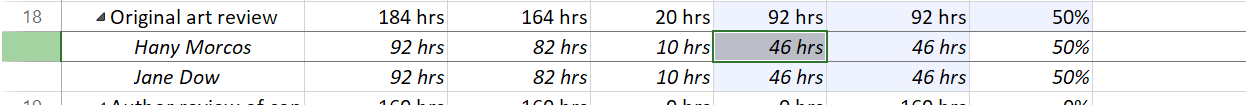
\includegraphics[width=0.9\textwidth]{./image/t5f2}
    \caption{Work Distribution}
\end{figure}
\begin{figure}[H]
    \centering
    
\includegraphics[width=0.9\textwidth]{./image/t5f3}
    \caption{Change Actual Work}
\end{figure}
\begin{figure}[H]
    \centering
    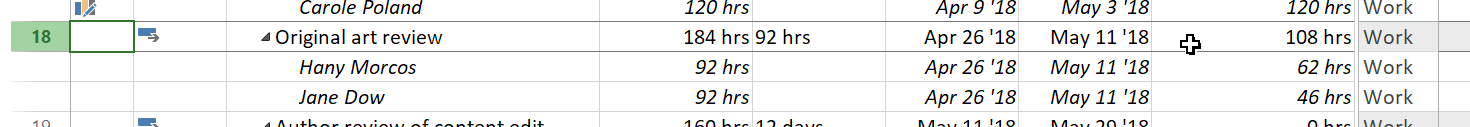
\includegraphics[width=0.9\textwidth]{./image/t5f4}
    \caption{Work Distribution}
\end{figure}

\subsection*{7. TrackTimephasedWork}
\begin{figure}[H]
    \centering
    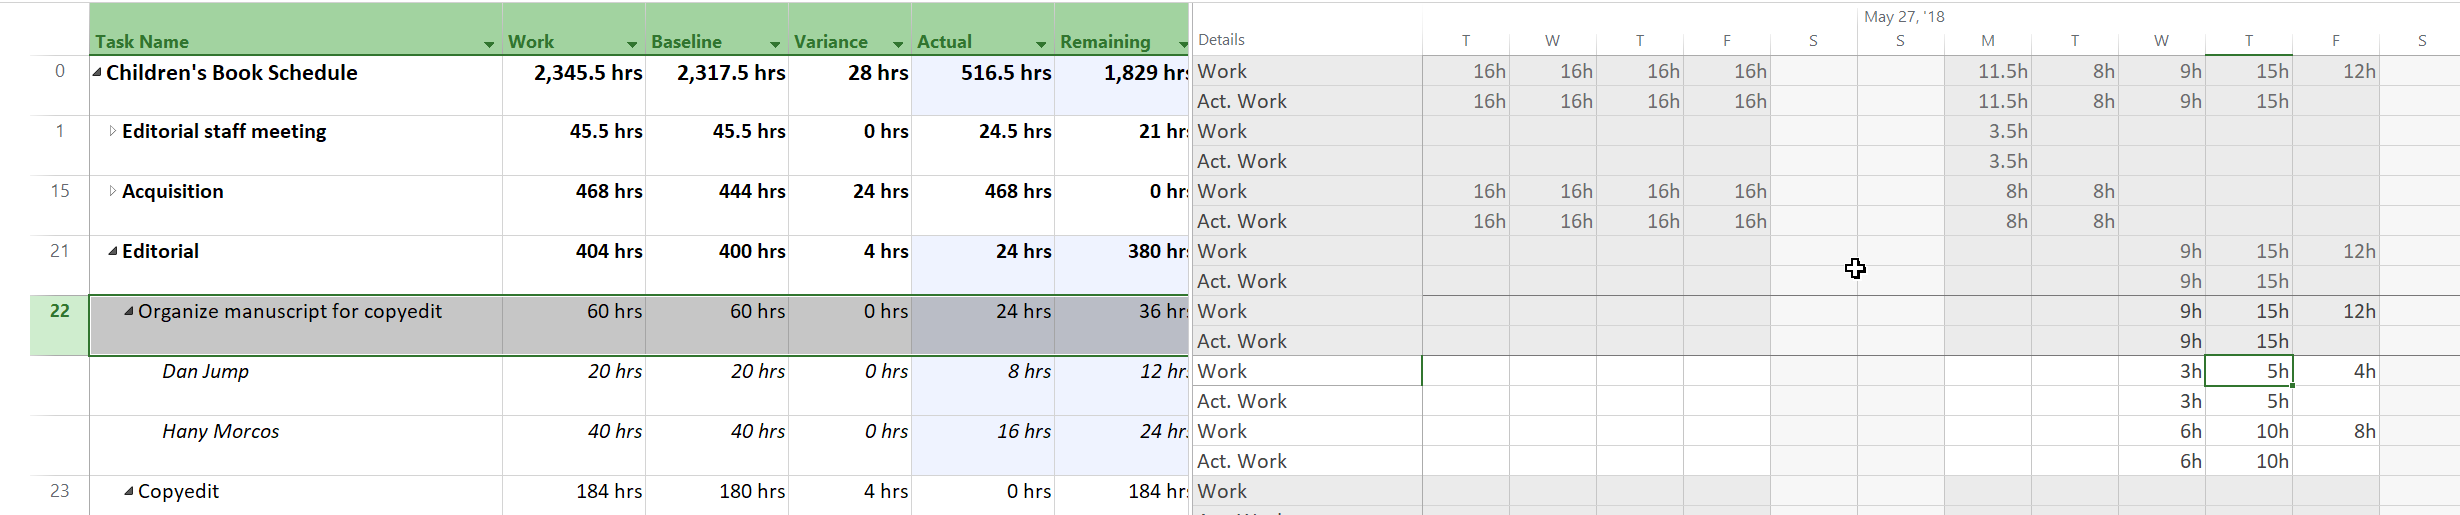
\includegraphics[width=0.9\textwidth]{./image/t6f1}
    \caption{Change Actual Work on May 30- May 31}
\end{figure}
\begin{figure}[H]
    \centering
    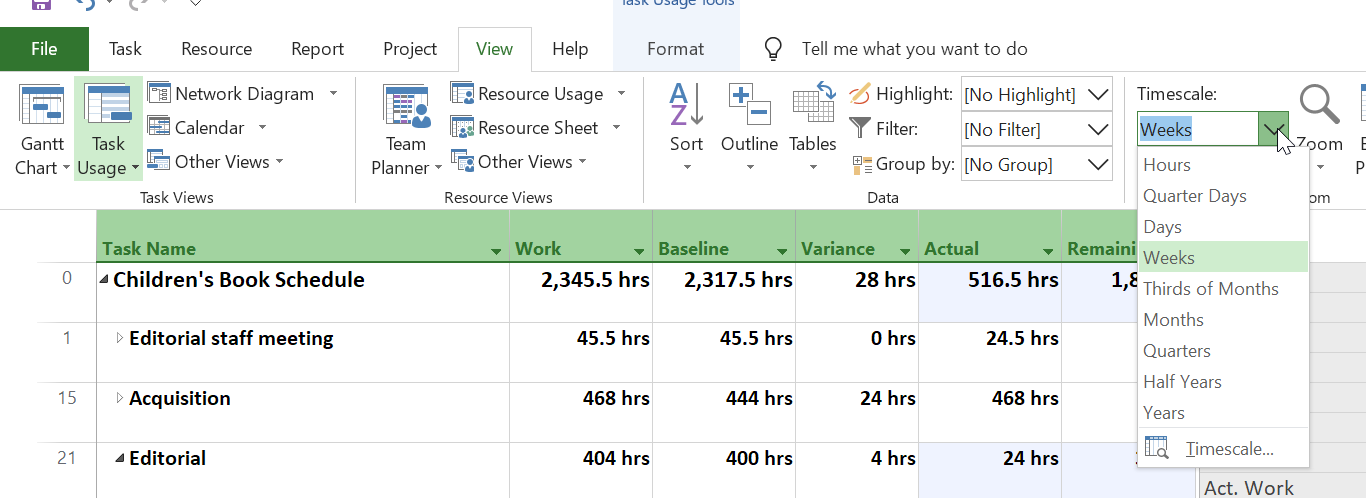
\includegraphics[width=0.9\textwidth]{./image/t6f2}
    \caption{Change Timescale}
\end{figure}
\begin{figure}[H]
    \centering
    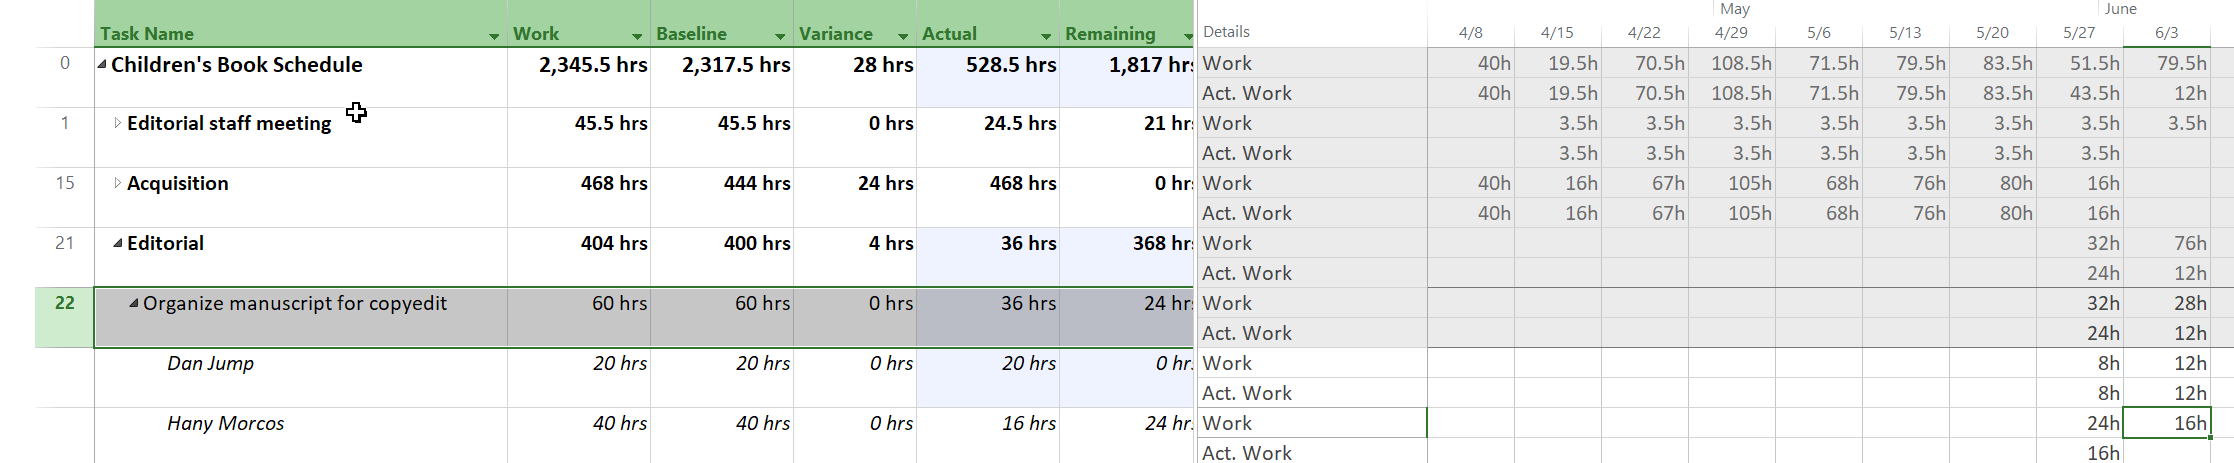
\includegraphics[width=0.9\textwidth]{./image/t6f3}
    \caption{Change Dan Jump's actual work}
\end{figure}

\subsection*{8. RescheduleIncompleteWork}
\begin{figure}[H]
    \centering
    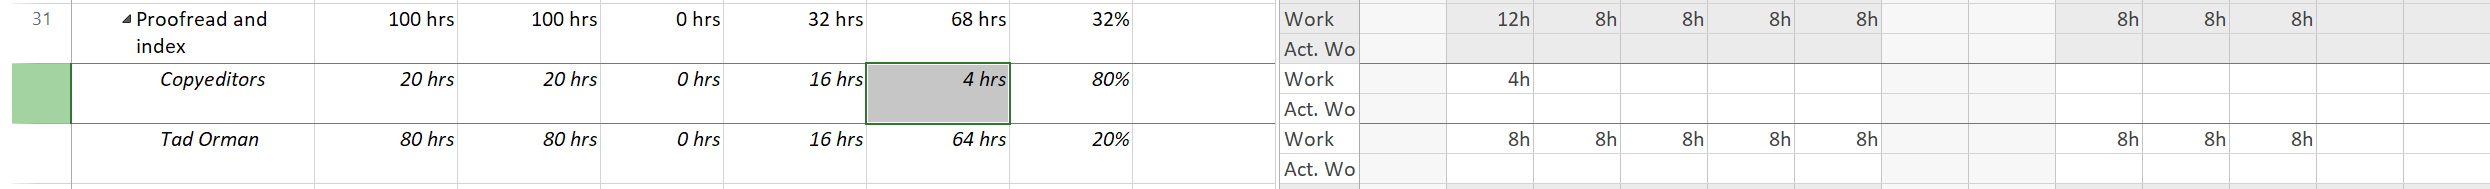
\includegraphics[width=0.9\textwidth]{./image/t7f1}
    \caption{a. Latest actual work recorded}
\end{figure}
\begin{figure}[H]
    \centering
    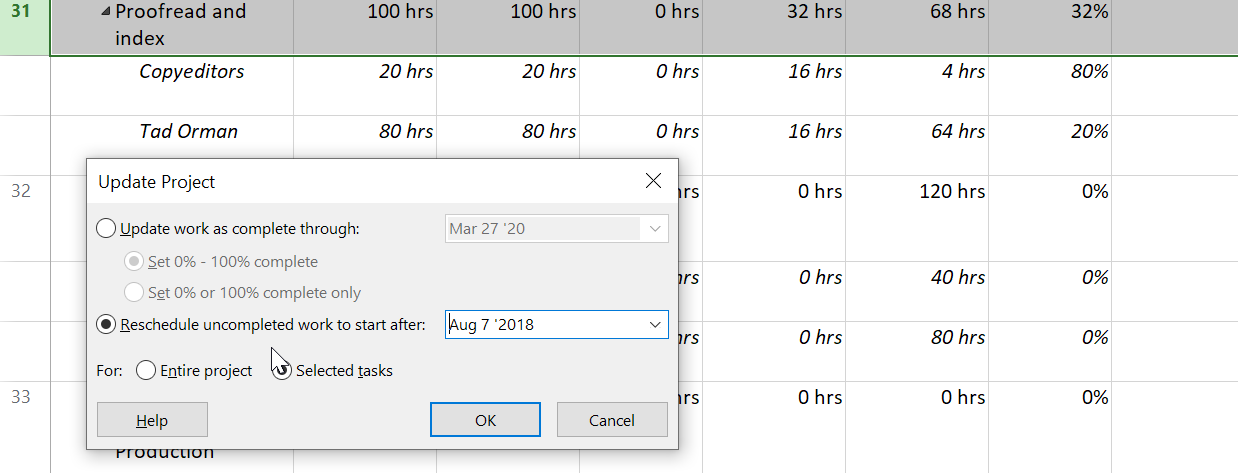
\includegraphics[width=0.9\textwidth]{./image/t7f2}
    \caption{b. Reschedule}
\end{figure}
\begin{figure}[H]
    \centering
    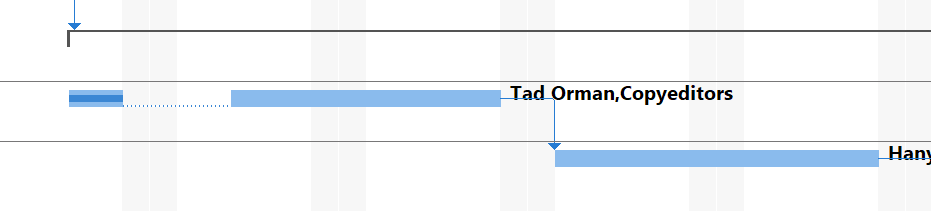
\includegraphics[width=0.9\textwidth]{./image/t7f4}
    \caption{b. Reschedule result}
\end{figure}
There is a gap in the task.
\end{document}
